\documentclass[qual, classic, a4paper]{ufbathesis}
\usepackage[utf8]{inputenc}
\usepackage[brazil]{babel}
\usepackage{fancyvrb}
\usepackage[alf]{abntex2cite}
\usepackage{graphicx}
\DeclareGraphicsExtensions{.pdf}

%\date{?? de Junho de 2016}
\adviser[f]{Profa. Dra. Christina von Flach G. Chavez}
\coadviser{Prof. Dr. Paulo Roberto Miranda Meirelles}

\title{
  Caracterização da qualidade interna de ferramentas de análise estática de
  código fonte
}
\author{Joenio Marques da Costa\\
  {\small joenio@joenio.me}
}

\begin{document}
\frontpage
\frontmatter
\presentationpage

%\acknowledgements
%DIGITE OS AGRADECIMENTOS AQUI
%
%\resumo
%DIGITE O RESUMO AQUI
%
%\begin{keywords}
%DIGITE AS PALAVRAS-CHAVE AQUI
%\end{keywords}
%
%\abstract
%RESUMO EM INGLÊS
%
%\begin{keywords}
%DIGITE AS PALAVRAS-CHAVE AQUI
%\end{keywords}

\tableofcontents
\listoffigures
\listoftables
\mainmatter

\chapter{Introdução}

(à fazer)

% falar aqui de ferramentas de análise estática e o porque escolhi elas? artigo
% com um reumo geral de ferramentas de analise: Source Code Analysis: A Road Map.pdf

\section{Contribuições esperadas}

(à fazer)

\chapter{Fundamentação teórica}

% 1 possibilitar replicar estudos é importante, referencia ciencia aberta, etc
% 
% 2 dentre as inúmeros requisitos para replicar temos o software/ferramenta que
% precisa estar disponível e ter qualidade mínima para ser re-utilizado
% 
% 3 para medir o quanto as ferramentas podem ser reutilizadas iremos medir a
% qualidade de software, interna e externa
% 
% 4 a qualidade interna será medida através de métricas de código-fonte
% 
% 5 os valores encontrados serão associados de alguma forma a caracteristicas de
% qualidade externa

\section{Engenharia de Software}

Sistemas de software são utilizados em praticamente todas as áreas do
conhecimento humano e têm exercido um papel essencial em nossa sociedade
\cite{Mafra2006}. A dependência crescente de serviços oferecidos por tais
sistemas evidencia a necessidade de produzir software de qualidade,
contornando os  desafios relacionados a funcionalidades incompletas ou
incorretas, custos acima do esperado ou prazos não cumpridos.

Diante destes desafios, surge a Engenharia de Software, uma disciplina
centrada no desenvolvimento de sistemas de software através
de uma abordagem sistemática, disciplinada, e quantificável para o
desenvolvimento, operação e manutenção \cite{SWEBOK2014}.

Nas últimas décadas, o foco em estudos empíricos na área de Engenharia de
Software tem crescido significantemente \cite{Stol2015}, resultando no uso
crescente de métodos como surveys, estudos de caso, experimentos e revisões
sistemáticas de literatura. Através destes estudos empíricos, pesquisadores
transformam a Engenharia de Software em uma disciplina mais científica e
controlável -- a  Engenharia de Software Experimental -- provendo meios para
avaliar e validar métodos, técnicas, linguagens e ferramentas.

Não raro, muitos destes estudos criam novos sistemas de software, tais
sistemas costumam ser utilizados como meio para atingir os resultados da
pesquisa ou, em alguns casos, são o próprio fim do estudo realizado. Neste
trabalho, tais ferramentas de software são nosso objeto de pesquisa e serão
chamados de "software científico" \ -- \citeonline{Portillo12} utiliza o termo
"research tool" para designar este mesmo tipo de software.

\section{Software científico}

Softwares científicos são ferramentas de software desenvolvidas no decorrer de
pesquisas científicas como parte do estudo realizado, podem ser pequenos
scripts, protótipos, ou mesmo softwares mais elaborados que demonstram ou
refletem os resultados de uma pesquisa. Em Engenharia de Software este tipo de
software desempenha um papel essencial e sua importância pode ser notada
através do grande número de conferências com sessões específicas para
publicação de ferramentas.

\citeonline{Kon2011} em um estudo sobre como pesquisas em Engenharia de
Software podem se beneficiar de informações disponíveis no ecosistema de
Software Livre fizeram uma análise de 10 edições do SBES\footnote{Brazilian
Symposium on Software Engineering} e concluíram que apesar do aumento do
interesse por parte dos pesquisadores em disponibilizar o código-fonte de suas
ferramentas isto ainda é minoria. O que confirma a preocupação de
\citeonline{Krishnamurthi2015} em um estudo sobre repetibilidade de pesquisas
científicas onde chamam atenção para o papel central que
os artefatos de software possuem em pesquisas de ciência da computação e
questionam: "Onde está o software nas pesquisas sobre linguagem de
programação?".

A partir daí, podemos então afirmar que softwares científicos são peça
fundamental para que pesquisadores independentes possam reproduzir, validar ou
expandir resultados encontrados em estudos e assim aumentar o rigor científico
de tais pesquisas \cite{Vitek2011}.

\section{Reprodutibilidade}

Reprodutibilidade é a habilidade de replicar um experimento ou estudo em sua
totalidade a fim de confirmar suas hipóteses, o termo apesar de ser
relativamente concensual entre as várias áreas da ciência possui algumas
divergências de uso, o que levou \citeonline{Feitelson2015} a propor as
seguintes definições:

\begin{description}
  \item[Repetição] Refazer exatamente o que outra pessoa fez usando os artefatos originais.
  \item[Replicação] Replicar com precisão exatamente o que outra pessoa fez, recriando os artefatos.
  \item[Variação] Repetir ou replicar exatamente o que outra pessoa fez, mas com alguma modificação controlada nos parâmetros.
  \item[Reprodução] Recriar o espírito do que outra pessoa fez, usando seus próprios artefatos.
  \item[Corroboração] Obter os mesmos resultados de outra pessoa, usando outros meios e procedimentos experimentais.
\end{description}

Dentre estes termos destacam-se reprodução e corroboração por serem os métodos
que realmente trazem progressos para a ciência apesar de ainda serem um
obstáculo. Diante disso \citeonline{Peng2011} sugere adotar soluções
intermediárias como repetição, replicação e variação, apenas isto já
garantiria uma grande melhoria sobre a situação atual onde muitos estudos
ainda sofrem de dificuldades de repetição \cite{Tang2016}.

Enquanto pesquisadores publicam artigos descrevendo e divulgando seus
resultados, é raro que façam o mesmo com toda a produção gerada durante a
pesquisa. A maioria dos componentes necessários para a reprodução dos
resultados de uma pesquisa -- por exemplo, código-fonte e dados -- usualmente
permanecem não publicados.

Isto se configura como uma barreira para a reprodutibilidade, e
consequentemente para a repetição, replicação e variação de estudos já que a
disponibilidade de código-fonte é o primeiro passo para que isto ocorra, como
pode ser visto no espectro de reprodutibilidade de \citeonline{Peng2011}
reproduzido aqui na Figura \ref{reproducibility-spectrum}.

\begin{figure}[h]
  \center
  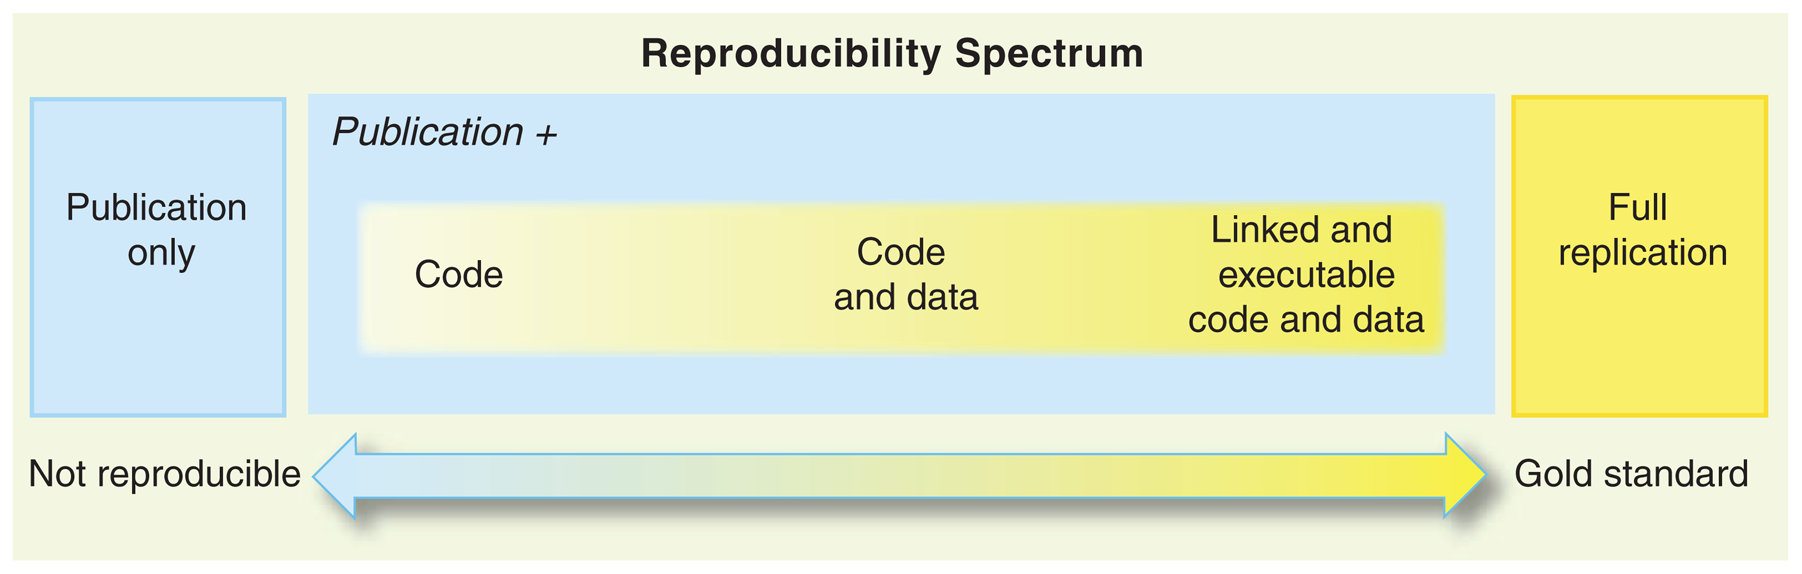
\includegraphics[scale=0.25]{imagens/reproducibility-spectrum.png}
  \caption{The spectrum of reproducibility\cite{Peng2011}}
  \label{reproducibility-spectrum}
\end{figure}

Dentro deste contexto, e considerando que pesquisas em engenharia de software
produzem bastante softwares científicos, surge a preocupação de avaliar a
qualidade de tais softwares a partir de métodos científicos adequados,
especialmente em relação a sua manutenabilidade e disponibilidade por serem
problemas comuns enfrentados pelos pesquisadores \cite{Prlic2012}.

\section{Qualidade de software}

Qualidade de software diz respeito à quão bem um software é projetado e o
quanto este software está em conformidade com o projeto, embora existam
inúmeras definições há concenso de que existem duas dimensões para se medir a
qualidade de um software, estas dimensões estão relacionadas à características
de qualidade interna e de qualidade externa.

Segundo \citeonline{McConnell2004}, qualidade interna são aquelas
características que preocupam o desenvolvedor, como: manutenabilidade,
flexibilidade, portabilidade, reusabilidade, legibilidade, testabilidade e
compreensão. São questões relacionadas ao código-fonte e em como o software
foi construído, como design e boas práticas por exemplo.

Qualidade externa são aquelas características que afetam o usuário, como por
exemplo: exatidão, usabilidade, eficiência, confiabilidade, integridade,
adaptabilidade, acurácia e robustez. Estas características impactam
extritamente no uso do software e não em como o software foi construído.

Segundo a ISO/IEC 25010 \cite{iso2011iec25010} estas características podem ser
divididas em subcaracterísticas. A característica usabilidade por exemplo é
dividida nas seguintes subcaracterísticas: capacidade de compreensão,
capacidade de aprendizado, operabilidade, atratividade e conformidade. Esta
caracteristica está relacionada a facilidade com que usuários aprendem e
utilizam um sistema, e passa por questões como facilidade de instalação,
aprendizado, e uso.

Sabe-se que, em algum nível, as caractarísticas de qualidade interna afetam as
características de qualidade externa \cite{McConnell2004}, softwares que não
possuem boa manutenabilidade por exemplo afetam a habilidade de correção de
defeitos, que por sua vez afetam as características de exatidão e
confiabilidade.

Dito isto podemos perceber que é possível inferir características de qualidade
externa de um software a partir de suas qualidades internas, o que pode ser
realizado a partir da análise de suas métricas de código-fonte.

\section{Métricas de código-fonte}

Uma métrica, segundo a definição da ISO/IEC 25010 \cite{iso2011iec25010}, é a
composição de procedimentos para a definição de escalas e métodos para
medidas, métricas de software costumam ser classificadas quanto aos critérios
utilizados para determiná-las ou quanto ao método de obtenção
\cite{Meirelles2013}, entre as classificações possíveis este trabalho dará
foco em métricas consideradas objetivas, ou seja, métricas que tratam de
características do código-fonte.

(desenvolver um pouco mais sobre métricas e fazer link com ferramentas para
análise e extração de métricas)

%, onde muitos trabalhos tentam correlacionar
%métricas de software com qualidade de software. (Subramanyam e Krishnan,
%2003) Briand et al.  (2000) (Zuse, 1990).
%Em suma, há uma variedade de métricas baseadas análise estática do
%código-fonte que permitem a avaliação de produtos de software (Gousios et al.,
%2007).

% Podemos afirmar então que podemos traçar algum
% nível de relação entre características de qualidade interna e externa.

\subsection{Ferramentas de análise estática de código-fonte}

(falar aqui de ferramentas de análise estática e extração de métricas)

\chapter{Metodologia}

%Com base nestas referências irei tomar alguns pontos básicos para contrastar
%com as ferramentas sendo anaalisadas a fim de caracterizar as mesmas em
%relação à um subcaracteristica básica externa, aquela à qual impacta em
%possibilitar qualquer outra, que é a capacidade de instalar e executar o
%software, partirei das seguintes questões:
%
%\begin{enumerate}
%  \item O software é fácil de instalar? (operability)
%  \item O software possui alguma instrução de instalação? (understandability ou learnability)
%  \item O software é facilmente encontrado para obtenção? (download, requisito para operability)
%  \item O software ao ser instalado devidamente executa suas funções mínimas sem erros? (compliance)
%\end{enumerate}
%
%As métricas de qualidade interna darão indícios de sua qualidade externa,
%especificamente em relação a caracteristicas de usabilidade, eu
%posso "ser cobaia" e tentar instalar cada ferramenta a ponto de medir a
%facilidade de instalação e uso. E isto será possível de correlacionar com as
%métricas de qualidade. Será?

Neste capítulo será apresentada a metodologia utilizada no estudo como meio
de validar as seguintes hipóteses:

\begin{enumerate}
  \item[{\bf H1:}] {\em Existem publicações sobre ferramentas de análise
    estática com disponibilidade de código-fonte}
  \item[{\bf H2:}] {\em Existem ferramentas de análise estática disponíveis
    livremente na indústria com disponibilidade de código-fonte}
  \item[{\bf H3:}] {\em Existem valores de referência para métricas de
    código-fonte para ferramentas de análise estática}
  \item[{\bf H4:}] {\em Ferramentas da indústria possuem melhores valores de
    métricas de código-fonte}
  \item[{\bf H5:}] {\em É possível relacionar a característica de qualidade
    externa usabilidade à valores de métricas de qualidade interna}
\end{enumerate}

% +\begin{itemize}
% +  \item Existe publicação sobre ferramentas de análise estática
% +  \item As publicações sobre ferramentas de análise estática disponibilizam o código fonte
% +  \item Existem ferramentas de análise estática disponíveis livremente na indústria
% +  \item O código fonte disponibilizado está (de fato) disponível livremente
% +  \item Existe similaridade em termos de métricas entre as ferramentas
% +  \item Existem valores de referência para métricas de código fonte
% +  \item As boas (?) ferramentas tem uma arquitetura semelhante
% +  \item É possível extrair uma arquitetura de referência a partir das ferramentas analisadas
% +  \item A arquitetura de referência gera um conjunto de métricas de referência
% +\end{itemize}
% +\section{Trabalhos relacionados}
%  
% +Pesquisas sobre o recente tópico, Ciência Aberta, \citeonline{Prlic2012} dão
% +dicas para o desenvolvimento aberto de software científico e citam que
% +disponibilizar o código criado durante pesquisas não apenas aumenta o impacto
% +como também se torna essencial para outros reproduzirem os resultados
% +encontrados. Eles citam ainda que manutenabilidade e disponibilidade do
% +software após a publicação é o maior problema enfrentado pelos pesquisadores
% +que desenvolvem tais softwares, e é aí que a participação no desenvolvimento
% +aberto desde o início pode trazer maior benefício.
%  
% +\citeonline{Portillo12} faz uma revisão sistemática caracterizando ferramentas
% +usadas em engenharia de software global, designa tais feramentas como
% +"research tool".
%  
% +\citeonline{Kon2011} cita que oftwares científicos são produtos de software e,
% +em geral, precisam ser avaliados com uso de métodos científicos adequados, e,
% +é de fundamental importância que estejam disponíveis e em funcionamento.

As seções à seguir descrevem as atividades de cada etapa da metodologia.

\section{Planejamento do estudo}

\subsection{Seleção das métricas}

\citeonline{Meirelles2013} realizou um estudo onde associou-se
qualidade do produto de software à qualidade de código através de métricas de
código-fonte como indicador para o sucesso de projetos de software livre.

(definir quais métricas serão utilizadas e justificar a escolha)

%este estudo selecionou algumas métricas de código-fonte como base, a partir de
%critérios como existência de valores de referência para as métricas, além de X
%Y e B. Aqui deste trabalho utilizaremos como base às mesmas métricas:
%
%\paragraph{Métricas de tamanho:}
%LOC (Lines of Code), AMLOC (Average Method LOC), Total Number of Modules or Classes
%
%\paragraph{Indicadores estruturais:}
%NOA (Number of Attributes), NOM (Number of Methods), NPA (Number of Public
%Attributes), NPM (Number of Public Methods), ANPM (Average Number of
%Parameters per Method), DIT (Depth of Inheritance Tree), NOC (Number of
%Children), RFC (Response For a Class), ACCM (Average Cyclomatic Complexity per
%Method)
%
%\paragraph{Métricas de acoplamento:}
%ACC (Afferent Connections per Class), CBO (Coupling Between Objects), COF
%(Coupling Factor)
%
%\paragraph{Métricas de coesão:}
%LCOM (Lack of Cohesion in Methods), SC (Structural Complexity)

\subsection{Seleção das fontes de ferramentas de análise estática}

Para ser possível validar as hipóteses aqui levantadas é necessário realizar
uma busca por ferramentas de análise estática desenvolvidas no contexto da
academia e da indústria, para isso, será feito um planejamento detalhado para
realizar a seleção de ferramentas em cada um destes contextos.

No contexto acadêmica a busca por ferramentas será feita
através de artigos publicados em conferências que tenham histórico de
publicação sobre ferramentas de análise estática de código fonte. Estes
artigos serão analisados e aqueles com publicação de ferramenta de análise
estática serão selecionados.

Na indústria a busca por ferramentas será feita a partir
de referências encontradas na internet, algumas organizações mantém listas de
ferramentas para análise de código-fonte, a Wikipedia também mantém uma lista
de ferramentas, estas referências serão utilizadas como ponto de partida e
cada ferramenta será analisada a fim de validar se são da indústria ou
surgiram em contexto acadêmico.

Uma vez que as ferramentas tenham sido selecionadas inicia-se a extração de
seus atributos de qualidade interna.

\subsection{Seleção da ferramenta de análise estática de código-fonte}

Para realizar a caracterização das ferramentas através dos seus atributos de
qualidade interna é necessário uma ferramenta capaz de analisar estaticamente
o código-fonte destas ferramentas e extrair atributos relacionados à sua
qualidade interna. Para isto utilizaremos o Analizo\cite{Terceiro2010}.

(falta justificar! quais vantagens? referencias?)

\section{Coleta de dados}

A partir das fontes selecionadas na etapa anterior serão realizadas duas
atividades para identificar e mapear as ferramentas de análise estática com
código-fonte disponível, uma atividade relacionada ao levantamento de
ferramentas da academia, outra atividade relacionada ao levantamento de
ferramentas da indústria.

\subsection{Ferramentas da academia}

A seleção de ferramentas será relizada através de uma revisão estruturada dos
artigos selecionados a partir das seguintes conferências:

\begin{itemize}
  \item ASE - Automated Software
    Engineering\footnote{http://ase-conferences.org}
  \item CSMR\footnote{A conferência CSMR tornou-se SANER - Software Analysis,
    Evolution, and Reengineering a partir da edição 2015.} - Conference on
    Software Maintenance and
    Reengineering\footnote{http://ansymore.uantwerpen.be/csmr-wcre}
  \item SCAM - Source Code Analysis and Manipulation Working
    Conference\footnote{http://www.ieee-scam.org}
  \item ICSME - International Conference on Software Maintenance and
    Evolution\footnote{http://www.icsme.org}
\end{itemize}

Chamamos de revisão estruturada um processo disciplinado para seleção de
artigos a partir de critérios bem definidos de forma que seja possível a
reprodução do estudo por parte de pesquisadores interessados. Alguns
resultados preliminares podem ser consultados na Tabela \ref{artigos-do-scam}
da Seção \ref{resultados}.

\subsection{Ferramentas da indústria}

A seleção de ferramentas da indústria será feita a partir de uma busca manual
em fontes encontradas na Internet sobre ferramentas de análise estática.

O projeto SAMATE\footnote{
http://samate.nist.gov} - {\em Software Assurance Metrics and Tool Evaluation}
disponível em \citeonline{SamateAnalysers} mantém uma lista de
ferramentas de análise estática mantida, mais sobre o projeto SAMATE pode
ser encontrado em \citeonline{Ribeiro2015}.

O software Spin mantém em seu site uma lista de ferramentas comerciais e de
pesquisa para análise estática de código-fonte para C em
\citeonline{spinSourceAnalysisTools}.

O Instituto de Engenharia de Software do CERT mantém uma lista de ferramentas
de análise estática em \citeonline{certSecureCodingTools}.

O software Flawfinder oferece em seu site um link com referências para
inúmeras ferramentas livres, proprietárias, gratuitas mas não-livres de
ferramentas de análise estática e outros tipos de análise em
\citeonline{wheelerStaticAnalysisTools}.

Uma outra fonte contendo uma relação expressiva de ferramentas é mantida na
Wikipedia em \citeonline{wikipediaListStaticCodeAnalysis}.

Estas fontes serão pesquisadas manualmente em busca de ferramentas de análise
estática que tenham sido desenvolvidas no contexto da indústria, algums
resultados preliminares podem ser encontrados nas Tabelas
\ref{ferramentas-do-nist-com-codigo} e \ref{ferramentas-do-nist-sem-codigo}.

\section{Caracterização dos artigos}

Caracterização dos papers analisados na revisão estruturada e caracterização
teórica do ecosistema das ferramentas da academia.

\section{Caracterização das ferramentas}

Será realizada uma caracterização prática das ferramentas, tanto acadêmica
quando da indústria, através da análise e extração de métricas de código-fonte
das mesmas.

% Resultado = Documentação com métricas de referência para ferramentas de análise estática.

\section{Exemplo de uso}

Por fim, os valores de métricas de referência encontradas serão utilizadas
como guia para refatorar a ferramenta Analizo.

(ler o TCC "Código Limpo e seu Mapeamento para Métricas de Código Fonte" onde
foi feito trabalho similar)

\chapter{Conclusão}

\section{Resultados preliminares}\label{resultados}

A Tabela \ref{artigos-do-scam} apresenta um resumo do número de artigos em
cada edição do SCAM e quantos artigos trazem publicação de ferramenta de análise
estática com código fonte disponível.

\begin{table}
\caption{Total de artigos analisados por edições do SCAM}
\centering
\begin{tabular}{| l | c | c |}
\hline
Edição    & Total de artigos & Artigos com ferramenta \\
\hline
SCAM 2001 & 23               & -                      \\
SCAM 2002 & 18               & -                      \\
SCAM 2003 & 21               & -                      \\
SCAM 2004 & 17               & -                      \\
SCAM 2005 & 19               & -                      \\
SCAM 2006 & 22               & 2                      \\
SCAM 2007 & 23               & 1                      \\
SCAM 2008 & 29               & -                      \\
SCAM 2009 & 20               & -                      \\
SCAM 2010 & 21               & 1                      \\
SCAM 2011 & 21               & 1                      \\
SCAM 2012 & 22               & 4                      \\
SCAM 2013 & 24               & -                      \\
SCAM 2014 & 35               & 1                      \\
SCAM 2015 & ?? (pendente)    & ?                      \\
\hline
Total     & 315              & 10                     \\
\hline
\end{tabular}
\label{artigos-do-scam}
\end{table}

As Tabelas \ref{ferramentas-do-nist-com-codigo} e
\ref{ferramentas-do-nist-sem-codigo} apresentam ferramentas do NIST após
avaliação inicial sobre disponibilidade do código-fonte. Das 54 ferramentas
apenas 19 tinham código fonte disponível.

% Todos foram baixados em "dataset/NIST".

\begin{table}
\caption{Lista de ferramentas do SAMATE - NIST com código fonte não disponível}
\centering
\begin{tabular}{| l | l |}
\hline
Ferramenta & Avaliacao  \\
\hline
ABASH                     & código não disponível \\
ApexSec Security Console  & código não disponível \\
Astrée                    & código não disponível \\
bugScout                  & código não disponível \\
C/C++test®                & código não disponível \\
dotTEST™                  & código não disponível \\
Jtest®                    & código não disponível \\
HP Code Advisor (cadvise) & código não disponível \\
Checkmarx CxSAST          & código não disponível \\
CodeCenter                & código não disponível \\
CodePeer                  & código não disponível \\
CodeSecure                & site offline \\
CodeSonar                 & código não disponível \\
Coverity SAVE™            & código não disponível \\
Csur                      & código não disponível \\
DoubleCheck               & código não disponível \\
Fluid                     & código não disponível \\
Goanna Studio and Goanna Central & código não disponível \\
HP QAInspect              & código não disponível \\
Insight                   & código não disponível \\
ObjectCenter              & código não disponível \\
Parfait                   & código não disponível \\
PLSQLScanner 2008         & código não disponível \\
PHP-Sat                   & link para código offline \\
PolySpace                 & código não disponível \\
PREfix and PREfast        & código não disponivel \\
QA-C, QA-C++, QA-J        & código não disponível \\
Qualitychecker            & código não disponível \\
Rational AppScan Source Edition & código não disponível \\
Resource Standard Metrics (RSM) & código não disponível \\
SCA                       & código não disponível \\
SPARK tool set            & código não disponível \\
TBmisra®, TBsecure®       & código não disponível \\
PVS-Studio                & código não disponível \\
xg++                      & código não disponível \\
\hline
\end{tabular}
\label{ferramentas-do-nist-sem-codigo}
\end{table}

\begin{table}
\caption{Lista de ferramentas do SAMATE - NIST com código fonte disponível}
\centering
\begin{tabular}{| l | l |}
\hline
Ferramenta & Avaliacao  \\
\hline
BOON                      & código disponível \\
Clang Static Analyzer     & código disponível \\
Closure Compiler          & código disponível \\
Cppcheck                  & código disponível \\
CQual                     & código disponível \\
FindBugs                  & código disponível \\
FindSecurityBugs          & código disponível \\
Flawfinder                & código disponível \\
Jlint                     & código disponível \\
LAPSE                     & código disponível \\
Pixy                      & código disponível \\
PMD                       & código disponível \\
pylint                    & codigo disponivel \\
RATS (Rough Auditing Tool for Security) & código disponível \\
Smatch                    & código disponível \\
Splint                    & código disponível \\
UNO                       & código disponível \\
Yasca                     & código disponível \\
WAP                       & código disponível \\
\hline
\end{tabular}
\label{ferramentas-do-nist-com-codigo}
\end{table}

Assim, temos um total de 19 ferramentas da indústria com código-fonte
disponível e ??? da academia com código fonte disponível, é preciso avaliar em
qual linguagem de programação foi escrita cada ferramentas pois só iremos
analisar aquelas em C, C++ ou Java que são suportadas pelo Analizo.

A ferramenta utilizada para identificar a linguagem de programação em que
estes softwares foram escritos foi a sloccount, uma ferramenta livre para
contagem de linhas de código fonte, onde se calcula em quais linguagens de
programação um software foi escrito.

%Abaixo destaco a linguagem de programação que tem maior
%porção em porcentagem.

Após analise ficamos com um total de 25 ferramentas, 15 da indústria e 10 da
academia, a Tabela \ref{total-de-ferramentas} traz um resumo de todos as
ferramentas analisadas.

\begin{table}
\caption{Lista com total de ferramentas a serem analisadas}
\centering
\begin{tabular}{| l | c | c |}
\hline
Ferramenta & Linguagem & Fonte \\
\hline
BOON                  & ansic                & industria \\
CQual                 & ansic                & industria \\
RATS                  & ansic                & industria \\
Smatch                & ansic                & industria \\
Splint                & ansic                & industria \\
UNO                   & ansic                & industria \\
Clang Static Analyzer & cpp                  & industria \\
Cppcheck              & cpp                  & industria \\
Jlint                 & cpp                  & industria \\
WAP                   & java                 & industria \\
Closure Compiler      & java                 & industria \\
FindBugs              & java                 & industria \\
FindSecurityBugs      & java                 & industria \\
Pixy                  & java                 & industria \\
PMD                   & java                 & industria \\
Indus                 & java                 & academia  \\
TACLE                 & java                 & academia  \\
JastAdd               & java                 & academia  \\
WALA                  & java                 & academia  \\
error-prone           & java                 & academia  \\
AccessAnalysis        & java                 & academia  \\
Bakar Alir            & java/ada/python      & academia  \\
InputTracer           & ansic                & academia  \\
srcML                 & cpp/cs (cs = C\# ?)   & academia  \\
Source Meter          & java                 & academia  \\
\hline
\end{tabular}
\label{total-de-ferramentas}
\end{table}

\section{Cronograma}

(à fazer)

\backmatter
\appendix
\bibliography{bibliografia}
\end{document}
